\title{On using AI tools}
\author{Daniel Bosk}
\institute{KTH EECS TCS}

\mode*

\begin{frame}
  \maketitle
\end{frame}

\begin{abstract}
  Several TCS members already use AI tools daily, but access is fragmented and uncoordinated: some
subscriptions are funded through GRU, some through FOFU, and some are paid out of pocket.
PhD students and researchers are increasingly asking how to get access.
This presentation surveys the available options---free GitHub Copilot Pro, paid subscriptions
(Claude Pro, Copilot Pro+, Claude Max), direct API access, and the department's Azure AI Foundry
service via IT---and proposes a simple three-step model for coordinated onboarding and procurement
at the TCS level.

\end{abstract}

\begin{frame}
  \only<presentation>{\tableofcontents[hideallsubsections]}
  \only<article>{\tableofcontents}
\end{frame}


\section{Current Situation}

Several TCS members already use AI tools regularly in their day-to-day work.
Daniel, Ric, and Alexander use them extensively for course development, grading feedback,
literature reviews, and other teaching and research tasks.
Dicander also uses them to some degree.
More recently, PhD students have started asking how to obtain access.
At present, however, funding is scattered: some subscriptions are covered by GRU, some by
individual FOFU grants, and some members pay out of pocket.

\begin{frame}
  \begin{block}{Current situation}
    \begin{itemize}
      \item Daniel, Ric, Alexander use AI tools \emph{daily}.
      \item Dicander and others use them to varying degrees.
      \item PhD students are asking how to get access.
      \item Funding is fragmented: GRU, FOFU, out-of-own-pocket.
    \end{itemize}
  \end{block}
\end{frame}


\subsection{The Challenge}

Because there is no department-level coordination, costs and workflows differ by person.
Some submit manual expense claims; others rely on a colleague's account.
There is no shared onboarding path, no agreed spending limits, and no mechanism to give
PhD students or new researchers access quickly.
As usage grows, this fragmentation will become increasingly costly and hard to manage.

\begin{frame}
  \begin{block}{The challenge}
    \begin{itemize}
      \item Should learn to work these tools to not be left behind.
      \item Need scalable solution to encompass all.
    \end{itemize}
  \end{block}

  \pause

  \begin{block}{Work in progress}
    \begin{itemize}
      \item Daniel, Ric and Alexander will run a workshop with the students.
      \item On 20th May at 10:15.
      \item Focus on how to use AI tools for learning.
      \item And prepare them for future work.
      \item Want to do something similar on TCS days in June for staff.
    \end{itemize}
  \end{block}
\end{frame}


\section{Available Options}

\subsection{Subscriptions}

Several subscription tiers exist, suitable for different levels of daily use.
All can be procured through Servicecenter (contact: Marlene): purchase directly, send the PDF
receipt once a year, and Servicecenter handles cost allocation.
Viggo and Elena attest.

\begin{frame}
  \begin{block}{Options: subscriptions}
    \begin{description}
      \item[Copilot Pro] Free for students and teachers via GitHub --- good 
        starting point, just need to register.
      \item[Claude Pro] \textasciitilde220\,EUR/year --- covers moderate daily 
        use.
      \item[Copilot Pro+] \textasciitilde390\,USD/year --- \(5\times\) quota of 
        Copilot Pro.
      \item[Claude Max 5x] 100\,EUR/month --- for heavy users, \(5\times\) 
        quota of Claude Pro.
      \item[Claude Max 20x] 200\,EUR/month --- for very heavy users, 
        \(20\times\) quota of Claude Pro.
    \end{description}
    \medskip
    \textbf{Procurement:} Ask Servicecenter to order, PDF receipt once a year 
    to them.
  \end{block}

  \begin{onlyenv}<2>
    \vspace{-4em}

    \begin{question}[Funding]
      Who should fund it?
    \end{question}
  \end{onlyenv}
\end{frame}

\begin{frame}
  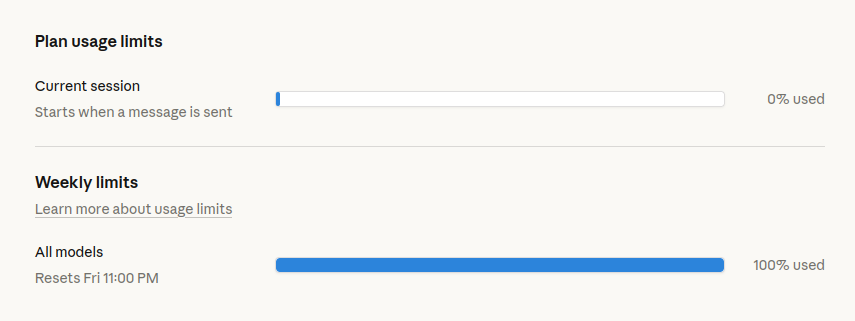
\includegraphics[width=\textwidth]{figs/claude-usage.png}
  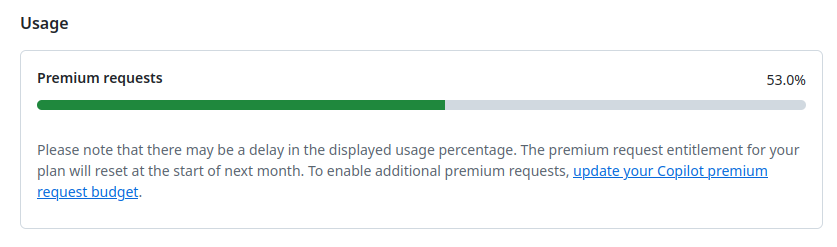
\includegraphics[width=\textwidth]{figs/copilot-usage.png}
\end{frame}

\subsection{API Access}

Beyond subscriptions, there are two paths for API-level access, which is needed for
experiments, automated course workflows, and student-facing tools.

Direct API access (e.g., via OpenAI or Anthropic) requires paying upfront and submitting
manual expense claims---cumbersome and error-prone.
Usage costs are low on average (roughly 200--300\,SEK/month, occasionally up to 1\,000\,SEK),
but the manual reimbursement process is a practical obstacle.

The alternative is Azure AI Foundry via KTH IT, which Martin's group already uses.
It supports sub-project budgets per user, internal invoicing (no expense claims), and spending
limits.
KTH IT requires a minimum commitment of approximately 4\,000\,SEK/month to cover their
administrative overhead.

\begin{frame}
  \begin{block}{Options: API access}
    \begin{description}
      \item[Direct API] Pay per use; manual expense claims;
      \item[Azure AI Foundry (IT)] Internal invoicing; per-user budgets and 
        limits;
        Martin's group uses it; requires \textasciitilde{}4\,000\,SEK/month 
        dept-wide
    \end{description}
  \end{block}

  \begin{remark}
    \begin{itemize}
      \item This is probably better for sparse bursts of use.
      \item And needed for experiments.
    \end{itemize}
  \end{remark}
\end{frame}

\begin{frame}
  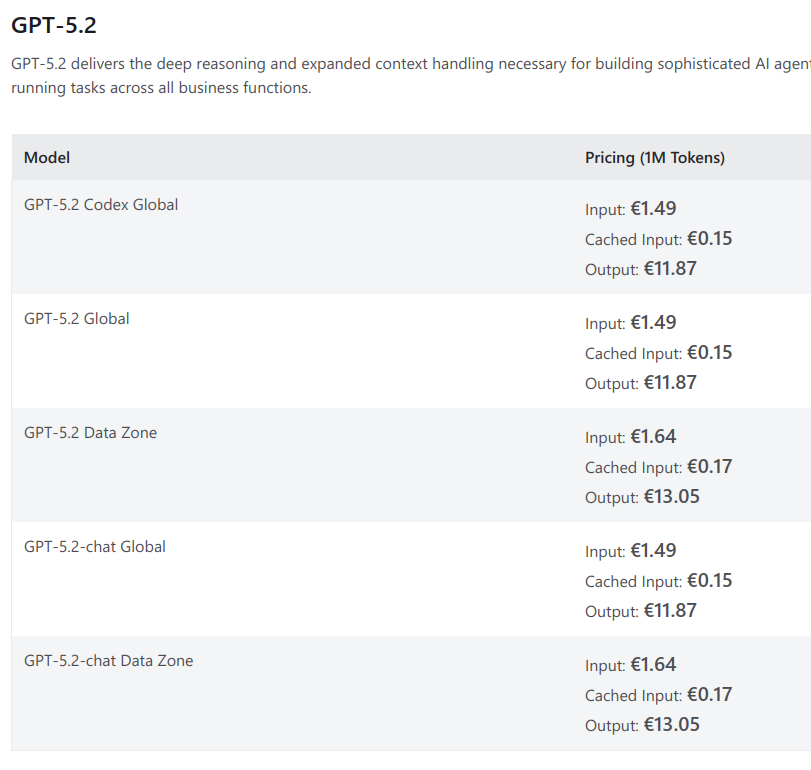
\includegraphics[height=0.9\textheight]{figs/azure-gpt-5.2-pricing.png}
\end{frame}


\section{Next Steps}

Several activities are already planned that support the rollout.

\begin{itemize}
  \item \textbf{20 May:} student-facing workshop on using AI in learning, run by Daniel, Ric,
    and Alexander.
  \item \textbf{June (TCS days):} a hands-on workshop for TCS staff showing practical use
    cases, allowing colleagues to decide whether a subscription is worthwhile for them.
  \item \textbf{After June:} assess interest in a department-wide Azure AI Foundry account;
    if enough users commit, this becomes cost-effective.
  \item \textbf{Immediate:} approve Copilot Pro+ subscription for Daniel
    (\textasciitilde{}390\,USD/year, funded via GRU).
\end{itemize}

\begin{frame}
  \begin{block}{Next steps}
    \begin{itemize}
      \item Get started using Github Copilot Pro (register!).
      \item \textbf{20 May} --- student workshop (Daniel, Ric, Alexander)
      \item \textbf{June (TCS days)} --- maybe a staff hands-on workshop?
      \item \textbf{Future} --- decide on dept-wide Azure AI Foundry, Claude 
        for Teams, or similar.
    \end{itemize}
  \end{block}
\end{frame}


\section{Demo}

\begin{frame}[fragile]
  \begin{minted}[breaklines]{text}
$ texgen -spacL CC -M slides -t "On using AI tools" -i ..
$ mutt # cat email from Elena to elena.email
$ opencode --prompt "Read elena.email and write draft slides in contents.tex."
$ vim contents.tex
  \end{minted}
\end{frame}

\begin{frame}[fragile]
  \begin{minted}{text}
$ llm chat -m kth-gpt-5.2 \
  -f <(canvaslms quizzes analyse -c prgi25 \
                                 -a "Delutvärdering")
Chatting with kth-gpt-5.2
Type 'exit' or 'quit' to exit
Type '!multi' to enter multiple lines, then '!end' to finish
Type '!edit' to open your default editor and modify the prompt
Type '!fragment <my_fragment> [<another_fragment> ...]' to insert one or more fragments
>
  \end{minted}
\end{frame}

\begin{frame}[fragile]
  \begin{minted}{text}
$ canvaslms assignments list -c vetcyb25h \
  -a Reflection
$ canvaslms submissions list -c vetcyb25h \
  -a Reflection.*models
$ canvaslms submissions view -c vetcyb25h \
  -a Reflection.*models \
  -u ^Only | less
$ claude "You can find the slides on the topic in CWD.
          You can read the students' reflections from the
          command canvaslms submissions view -c vetcyb25h
          -a Reflection.*models. Please adapt the slides to
          the students' misconceptions and weak points."
  \end{minted}
\end{frame}

\begin{frame}[fragile]
  \begin{minted}{text}
$ scholar rq \
  "What has the research on the Signal protocol focused
   since 2020?" \
  -n "Signal research full" -p wos -p ieee -p arxiv
$ scholar sessions resume "Signal research full"
$ for n in $(seq 5); do \
    scholar llm classify "Signal research full" -n 20 \
    scholar sessions resume "Signal research full" \
  done
$ scholar llm synthesize "Signal research full" \
  -o signal-survey.tex -f latex
$ latexmk -xelatex -pdf signal-survey.tex
$ scholar sessions export "Signal research full" \
  -f latex -o signal-survey-protocol.tex
$ latexmk -xelatex -pdf signal-survey-protocol.tex
  \end{minted}
\end{frame}
